\section{The sphere}
\label{sec:sphere}

We begin with the unit sphere, for which the Mie series provides the exact scattered field. The incident wave \eqref{eq:planewave} travels in the direction $\bd = (0,0,-1)^\top$ and is polarised along $\bp = (0,1,0)^\top$. We use this wave for all shapes unless stated otherwise. The wavenumber is $k = 2\pi$, so the sphere is two wavelengths across.

\subsection{Layout and convergence}

The sources are $N$ electric dipoles on the sphere of radius $R<1$, at the points of a Fibonacci lattice, with three unknown components each. The collocation points are the $M = 2N$ points of a Fibonacci lattice on the unit sphere, with equal weights. This gives $4N$ equations for $3N$ unknowns.

\autoref{fig:sphere} shows the error \eqref{eq:fielderror} against the Mie series. For $R = 0.5$ and $k = 2\pi$ the error is $2.7\times10^{-3}$ with $N = 100$ sources, $2.0\times10^{-9}$ with $N = 400$ and $2.4\times10^{-14}$ with $N = 1200$. The decay is not exponential in $N$. Plotted against $\sqrt{N}$ the curves are straight lines, so the error behaves like $\exp(-c\sqrt{N})$. This is the expected rate in three dimensions. A set of $N$ points on a sphere resolves spherical harmonics up to a degree proportional to $\sqrt{N}$, and the contribution of the harmonics beyond that degree decays geometrically with the degree. In two dimensions the same argument gives the rate $\exp(-cN)$ that Barnett and Betcke prove for the disc \cite{barnett2008}.

The scattered field of the sphere continues analytically up to the centre, so every radius $R$ encloses the singularity and every radius converges. The rate depends on $R$. A smaller radius converges faster, as the first two columns of \autoref{fig:sphere} show for $R = 0.3$ against $R = 0.9$. The price is the size of the coefficients. The right column shows that the norm of the coefficient vector grows as $R$ decreases, from order one at $R = 0.9$ to $10^{10}$ at $R = 0.1$ for $N = 400$. Large coefficients of alternating sign cancel in the sum \eqref{eq:mfs}, and the digits lost in the cancellation limit the accuracy. For $R = 0.3$ the error stalls at $2\times10^{-12}$. The best radius for $N = 400$ is about $0.35$ at $k = 2\pi$ and $0.45$ at $k = 4\pi$. We use $R = 0.5$, which is close to the best choice at both wavenumbers and reaches $10^{-12}$ or better.

\begin{figure}[htbp]
  \centering
  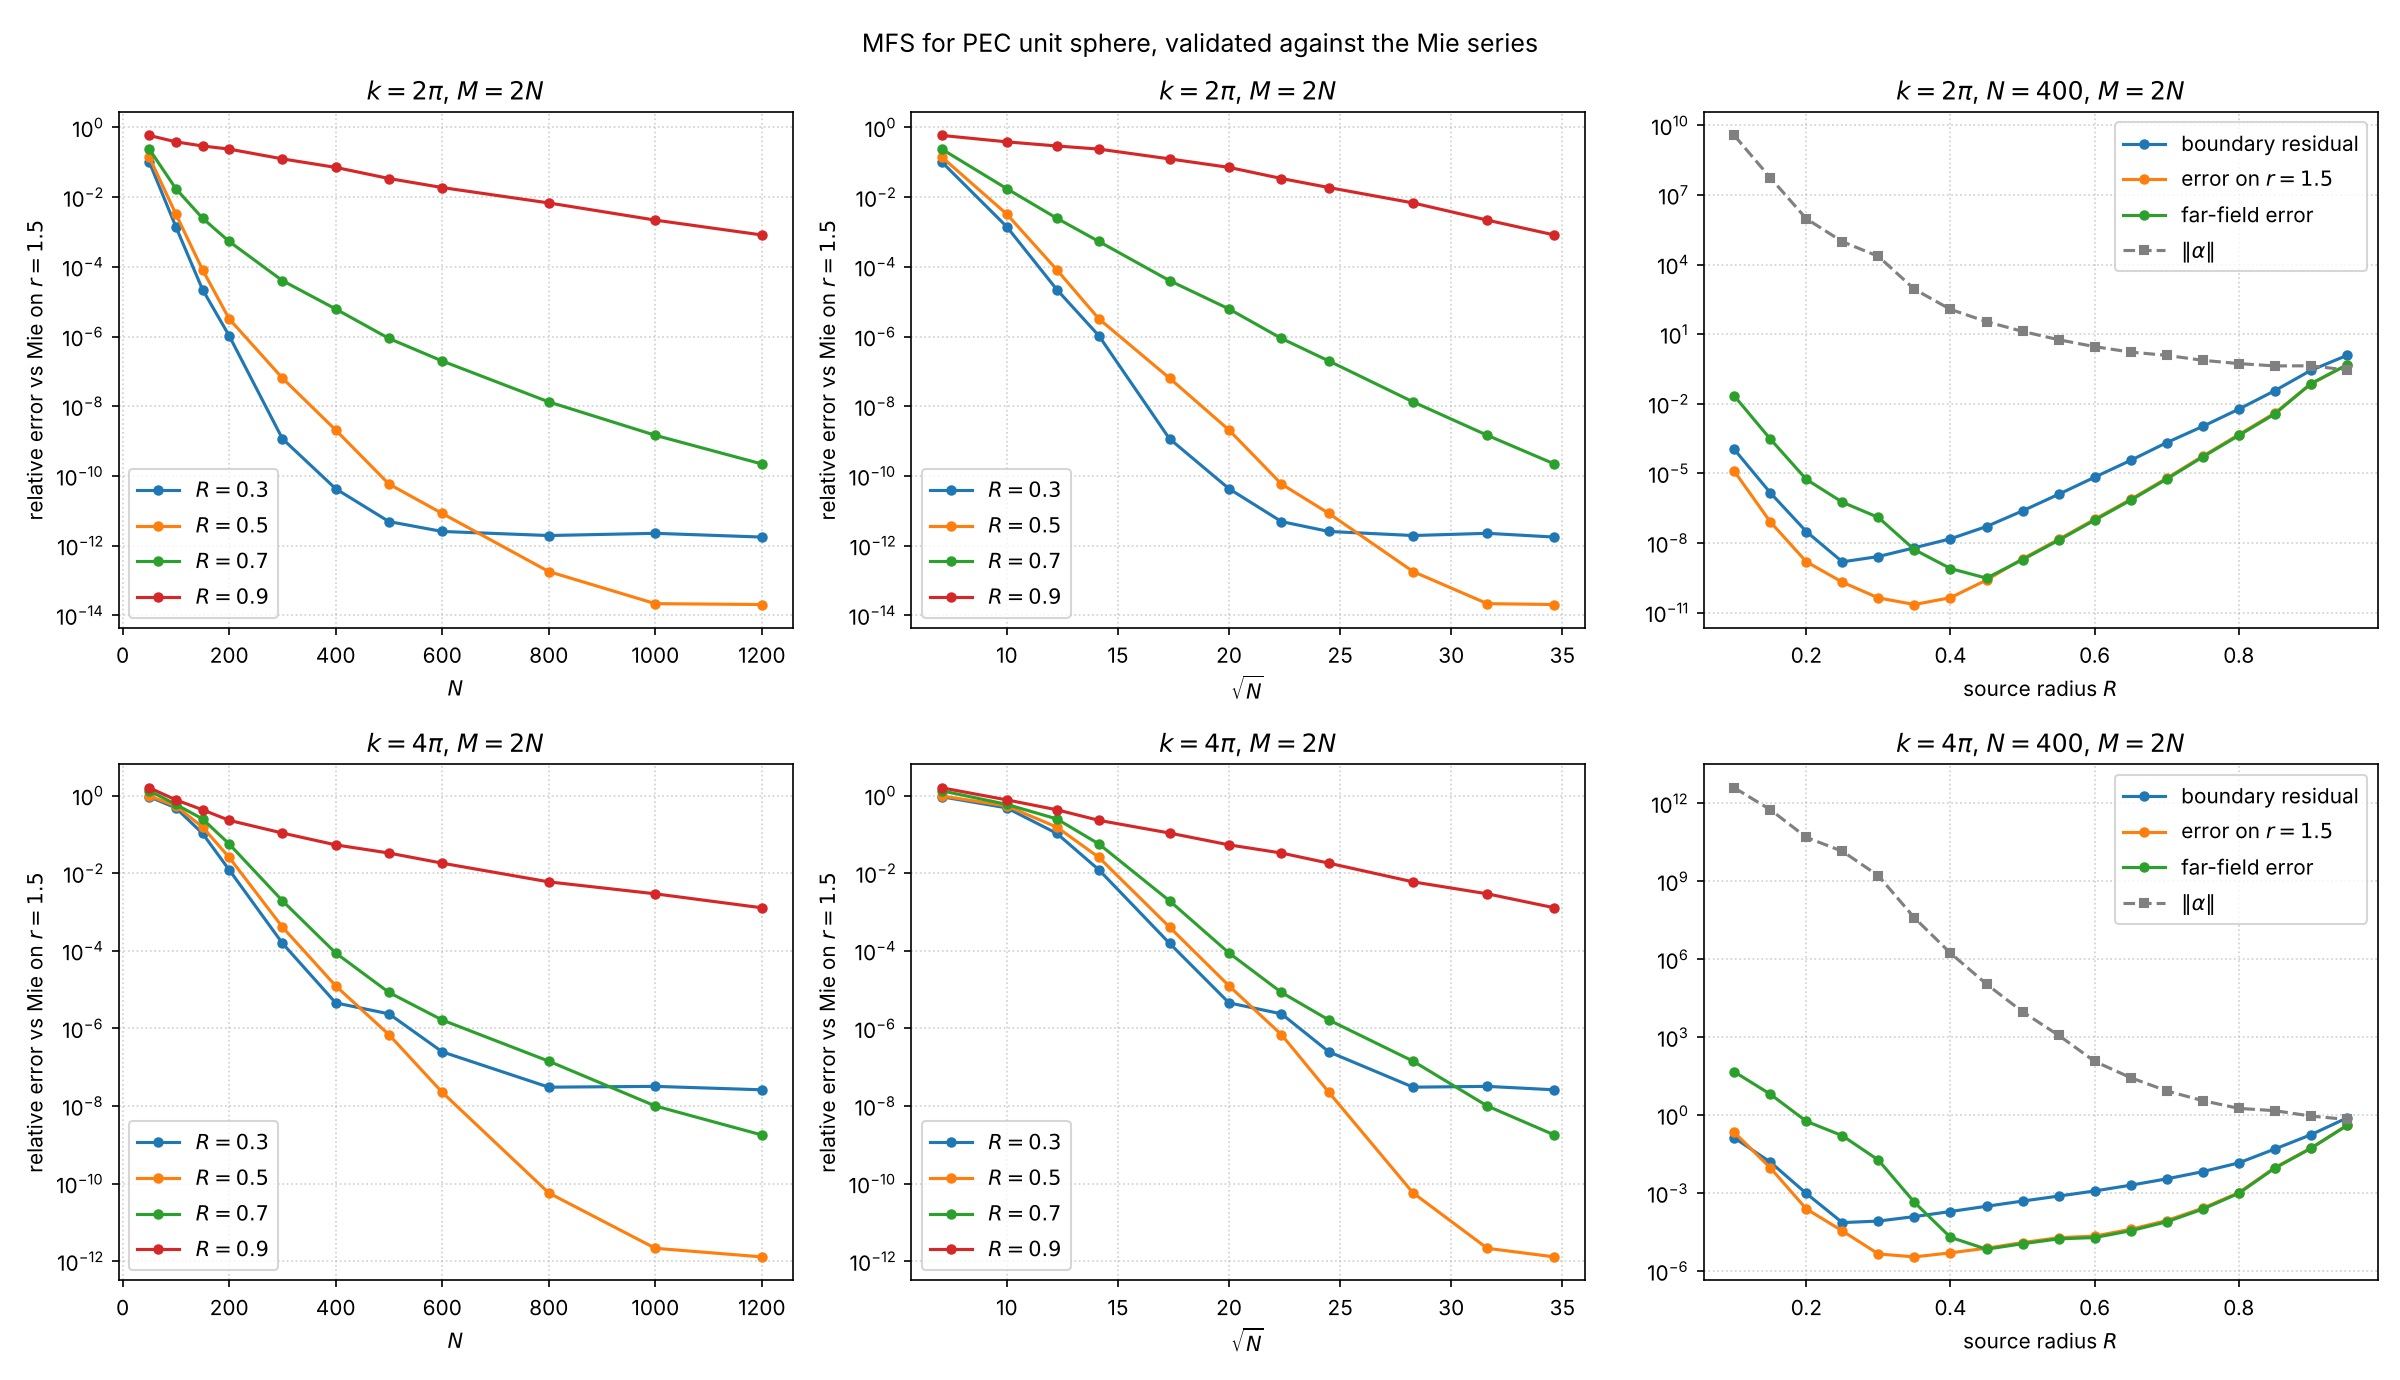
\includegraphics[width=\textwidth]{pec_sphere_convergence.png}
  \caption{Perfectly conducting unit sphere, error against the Mie series. Left: error against the number of sources $N$ for four source radii $R$. Centre: the same against $\sqrt{N}$. Right: error, boundary residual and coefficient norm against $R$ for $N = 400$. Top row: $k = 2\pi$. Bottom row: $k = 4\pi$.}
  \label{fig:sphere}
\end{figure}
%% TODO: redraw this figure in the style of the cost figures (it still carries
%% a title and the default colours); the data are in pec_sphere_convergence.py.

\subsection{Dependence on the wavenumber}

We repeated the experiment with $R = 0.5$ for $k = 4\pi$, $6\pi$ and $8\pi$, for which the sphere is four, six and eight wavelengths across. Interpolating between the runs, an error of $10^{-6}$ needs about $220$, $470$, $800$ and $1630$ sources at $k = 2\pi$, $4\pi$, $6\pi$ and $8\pi$. For the three larger spheres this is between $21$ and $28$ unknowns per square wavelength of surface. The number of unknowns thus grows in proportion to the surface area measured in wavelengths, as it must, and the constant is small. At $k = 8\pi$ the run with $1600$ sources takes $9$\,s. With more sources the error at this wavenumber stalls near $3\times10^{-9}$, because the coefficients grow as described above.

\subsection{Cost}
\label{sec:spherecost}

\autoref{tab:sphere} and \autoref{fig:costsphere} compare the MFS with Bempp. With $1200$ unknowns the MFS reaches an error of $2.0\times10^{-9}$ in $0.34$\,s. Bempp reaches $3.7\times10^{-3}$ with $9750$ unknowns in $26$\,s. Its error halves when the number of unknowns doubles, which is the rate of a lowest-order method on a surface approximated by flat triangles. Neither method uses the symmetry of the sphere.

The comparison is between a spectrally accurate method and a low-order one, and on a smooth body the outcome is not surprising. A boundary element method of high order on curved elements would converge much faster than Bempp does here. We include the sphere because it calibrates both codes against an exact solution.

\begin{table}[htbp]
  \centering
  \caption{Unit sphere, $k = 2\pi$: unknowns, wall time and error against the Mie series. MFS with $R = 0.5$; Bempp on quasi-uniform meshes.}
  \label{tab:sphere}
  \begin{tabular}{lrrl}
    \toprule
    Method & Unknowns & Time [s] & Error \\
    \midrule
    MFS   & 300 & 0.04 & $2.7\times10^{-3}$ \\
    MFS   & 600 & 0.10 & $2.7\times10^{-6}$ \\
    MFS   & 1200 & 0.48 & $2.0\times10^{-9}$ \\
    MFS   & 2400 & 2.2 & $1.7\times10^{-13}$ \\
    MFS   & 3600 & 5.9 & $2.3\times10^{-14}$ \\
    \midrule
    Bempp & 1269 & 0.78 & $3.2\times10^{-2}$ \\
    Bempp & 2733 & 3.5 & $1.4\times10^{-2}$ \\
    Bempp & 4824 & 7.8 & $7.6\times10^{-3}$ \\
    Bempp & 9750 & 33 & $3.7\times10^{-3}$ \\

    \bottomrule
  \end{tabular}
\end{table}

\begin{figure}[htbp]
  \centering
  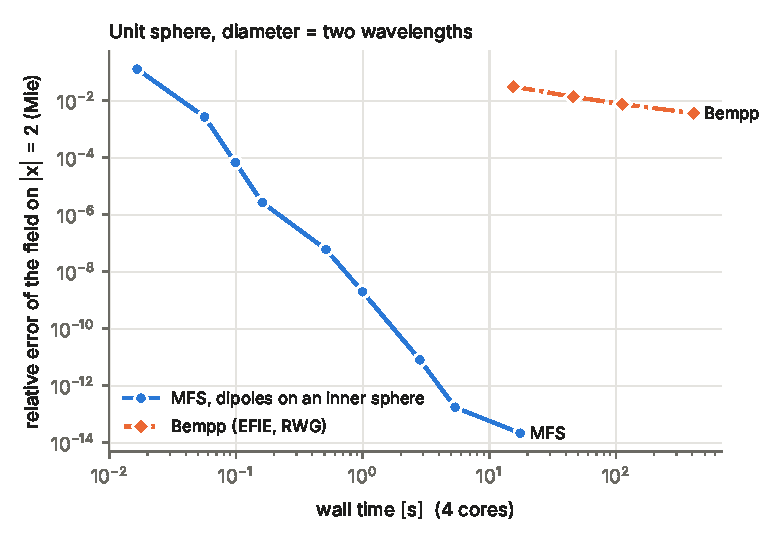
\includegraphics[width=0.62\textwidth]{fig_cost_sphere.pdf}
  \caption{Unit sphere, $k = 2\pi$: error against the Mie series as a function of wall time on four cores.}
  \label{fig:costsphere}
\end{figure}
